\chapter{Results}
\label{results}

The behaviour of the alternative FPGA solution needs to accurately replicate the behaviour of the existing microcontroller solution. There are two behavioural processes which were implemented by the prototype: the behaviour for a successful movement from one position to another and the regulation process which limits the current. The first of these scenarios occurs during normal operation to transfer the connection from one power supply to another. The regulation process must be used to limit the motor current in the event of a stalled or blocked motor. As part of the results for this project, the behavioural response to each of these scenarios is compared. 
The motor control function is compared between the two solutions in Section \ref{atys-movement}. The response of the current regulation process is compared in Section \ref{current-reg}. 

The motor control process output is a PWM signal of a duty-cycle which is calculated and generated by the ATyS processor. This duty-cycle value is compared for each of the solutions as part of the results. Additionally, the motor current is also displayed and compared which represents the response of the motor. For each of these tests, the data was taken directly from the Oscilloscope. One million points were taken over five seconds for each reading. The duty-cycle calculations were performed in Excel using the times between the rise and fall of the supplied signal.

\section{Experimental Setup}

\begin{figure}[h]
\centering
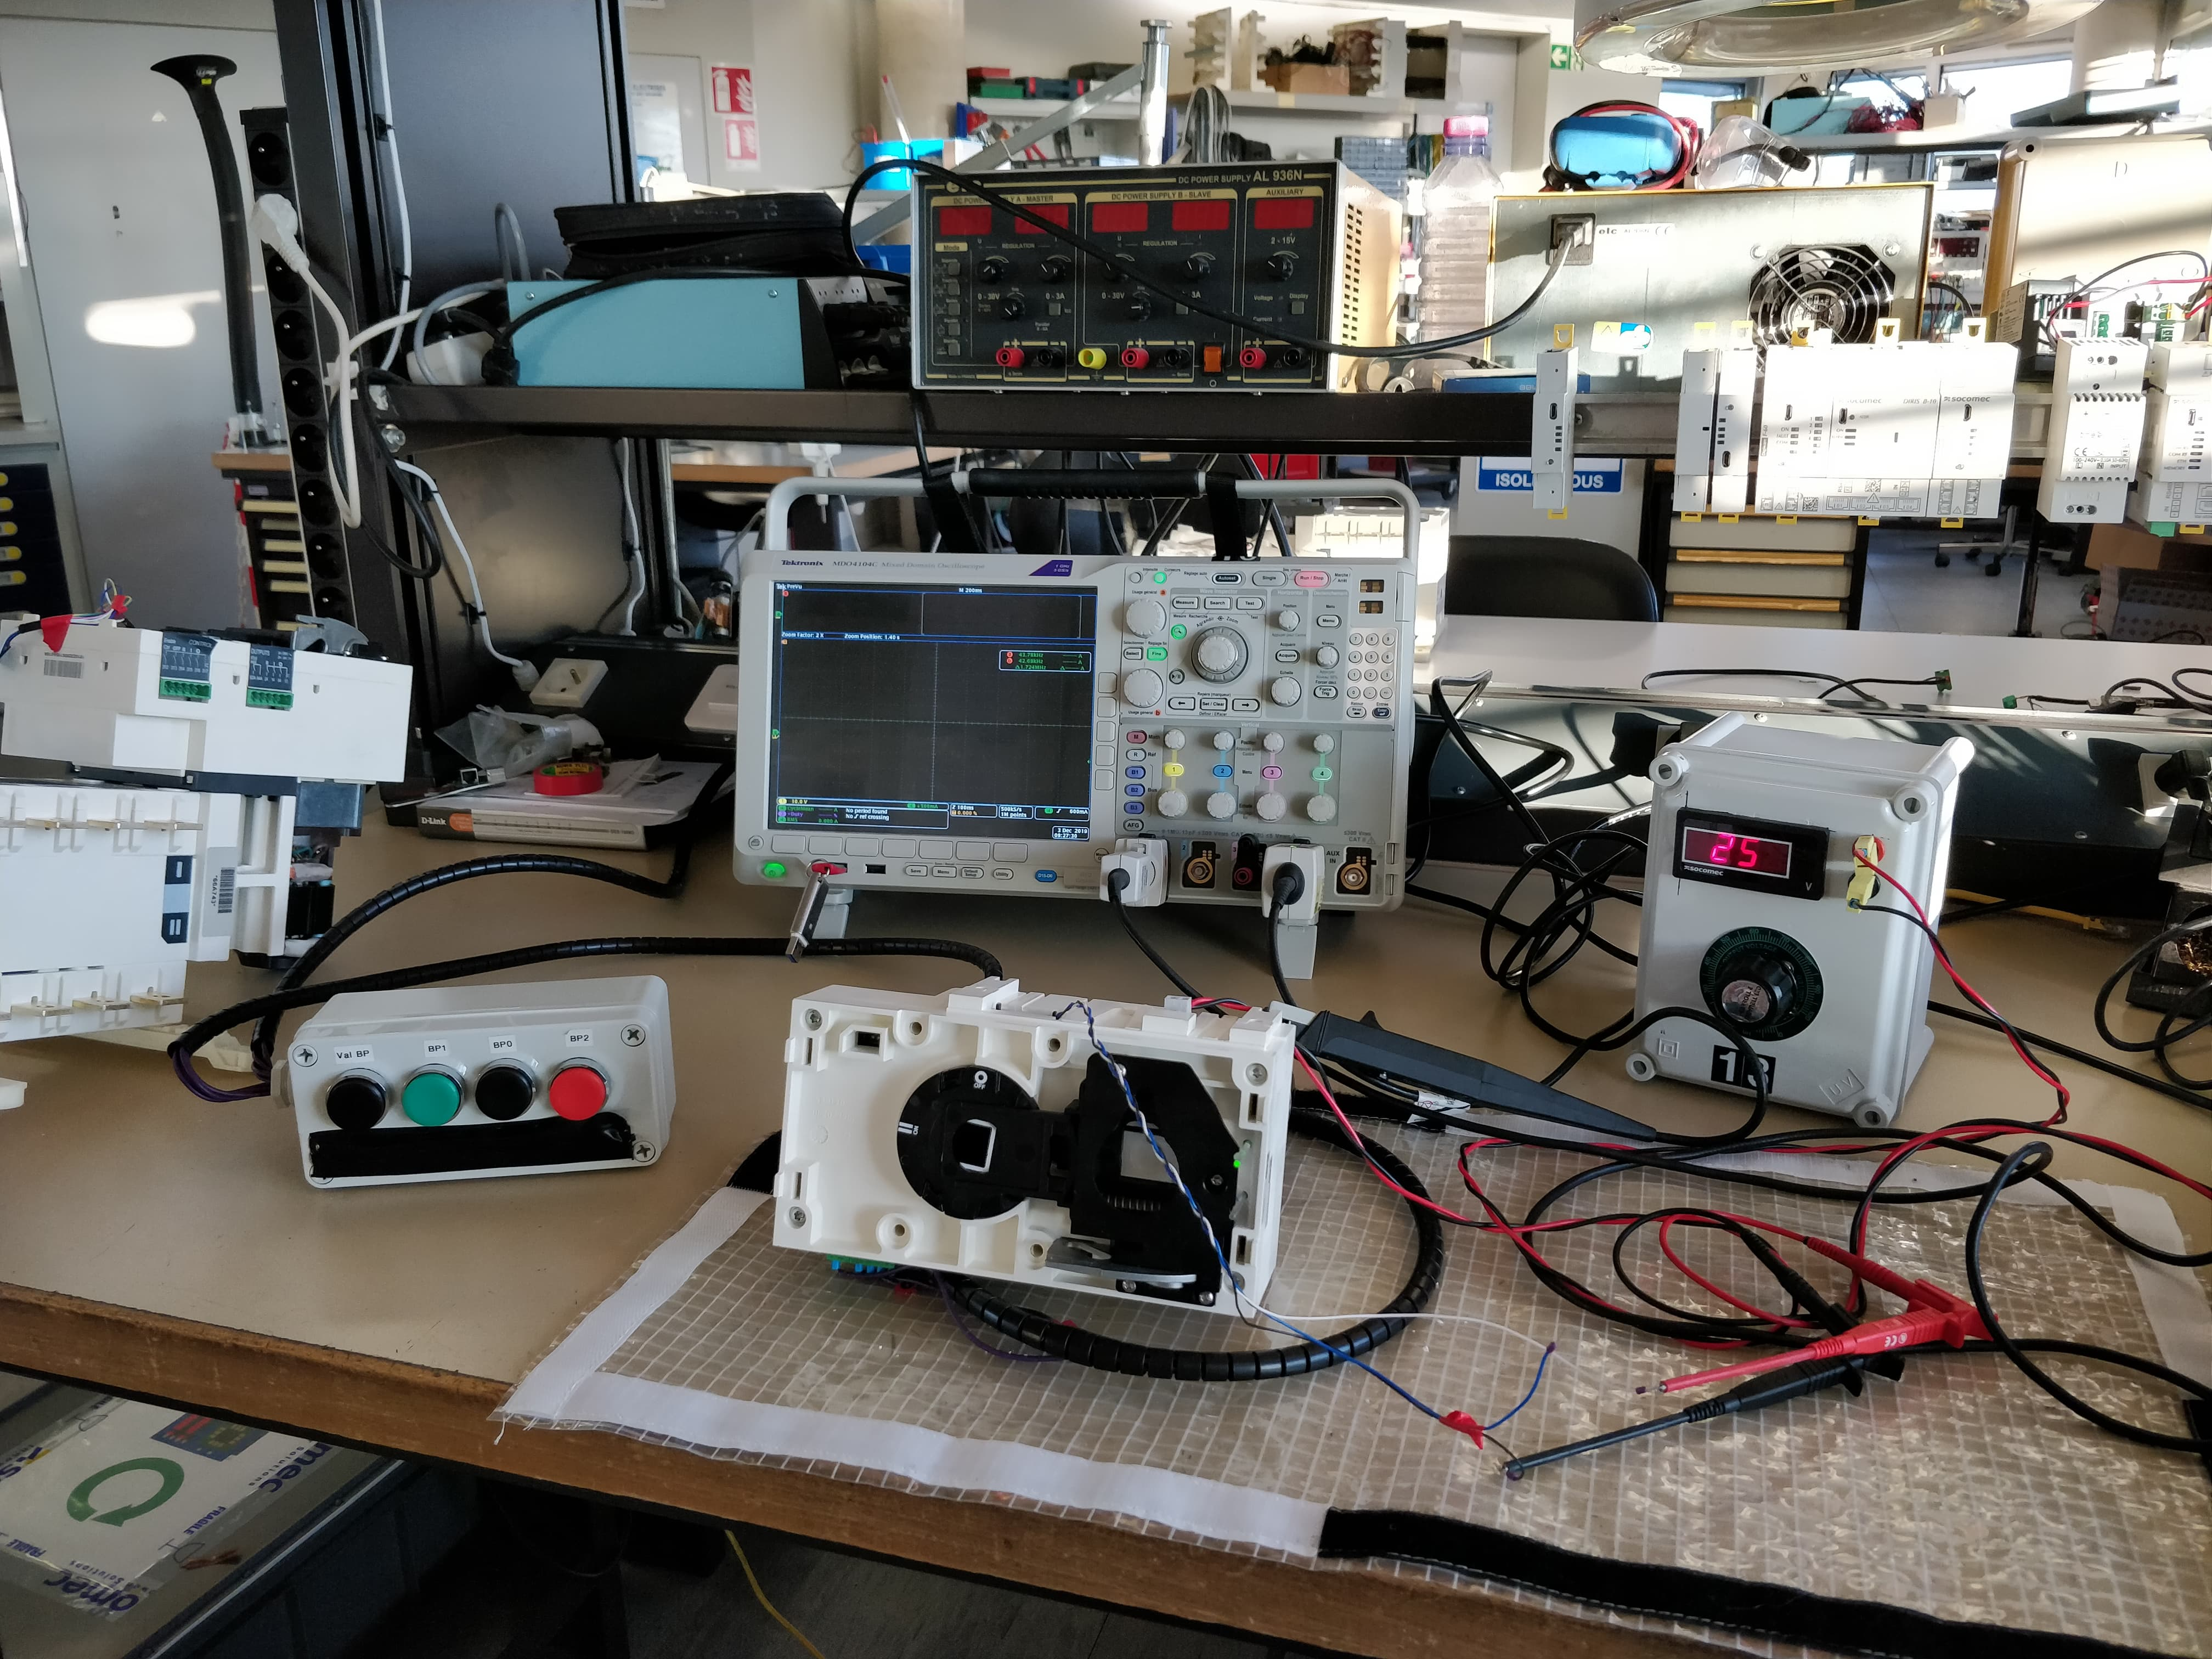
\includegraphics[width=\textwidth]{images/AtysExperimentalSetup.jpg}
\caption{The experimental setup for the FPGA vs microcontroller comparisons}
\label{atys_experimental_setup}
\end{figure}

The experimental setup for each of the tests can be seen in Figure \ref{atys_experimental_setup}. The equipment used for this experiment included an AC power supply, an oscilloscope, an ATyS casing and an ATyS command interface. Each of the PCB solutions being compared were placed into the same model of ATyS casing for experimentation. The oscilloscope had two inputs for each of the experiments: the motor current which was measured from the connection between the rotor and the stator, and the voltage supply to the IGBTs which was measured directly on the PCB. The supply voltage was set to 250V for the motor movement test and was reduced to 200V for testing the regulation processes. The same model of motor was used for both the FPGA and microcontroller boards. For the stalled motor test, the rotor from one motor was connected to the stator of the other to prevent any movement.
The same ATyS switch, the load for the motor, was used for each set of results. 

\section{ATyS Movement Test}
\label{atys-movement}

The core functionality which had to be replicated by the design in this project is the motor control of the ATyS system. This safety function allows the power supply connection to be transferred. The first test will be a comparison between how each of the processors, microcontroller and FPGA, perform this core activity. 

As described in the design section, the motor control processes follow a number of defined phases which determine the PWM provided to the motor. 
The motor control contains five discrete phases: PWM startup, PWM minimum, PWM increase, PWM regulation and braking. These phases are represented as states in a state machine in the FPGA design code which is shown in Appendix Item \ref{pwm-state-machine-code}. The stimulation of the motor during the control process has been defined for previous iterations of the ATyS device. An initial startup phase is used in order to activate the IGBTs and Thyristors required. The PWM, which supplies the IGBTs, is then set to the minimum for a short period before being increased to the maximum calculated value. This value is held until the required motor position is reached. At this point, braking is applied to each of the IGBTs. The results of the test, which involved the movement from position one to position two, are shown in Figure \ref{movement_test}.

\begin{figure}
\centering
\begin{subfigure}{0.8\textwidth}
\centering
\begin{tikzpicture}
%\pgfplotsset{scale only axis, scaled x ticks=base 10:3, xmin=0, xmax=0.06}

% current
\begin{axis}[
    %legend pos=south west,
  legend style={at={(0.5,0.03)},anchor=south},
  axis y line*=right,
  axis x line=none,
  ymin=-2, ymax=2,
  ylabel=Motor Current (A)
]

\addlegendimage{/pgfplots/refstyle=Duty_Cycle}\addlegendentry{Duty-cycle}
\addplot[red!60]table {Graphs/MicroMovement/MotorCurrent.txt};
\addlegendentry{Motor Current}
\label{Motor_Current}
\end{axis}

% pwm
\begin{axis}[
axis y line*=left,
ymin=-10, ymax=110,
xlabel=Time (s),
ylabel=PWM Duty-cycle (\%),
]
\addplot[blue!80]table {Graphs/MicroMovement/DutyCycle.txt};
\label{Duty_Cycle}
\end{axis}


\end{tikzpicture}

\subcaption{Micro-controller Motor Control}
\label{MICROgraph}
\end{subfigure}

\begin{subfigure}{0.8\textwidth}
\centering
\begin{tikzpicture}
%\pgfplotsset{scale only axis, scaled x ticks=base 10:3, xmin=0, xmax=0.06}

% current
\begin{axis}[
    %legend pos=south west,
  legend style={at={(0.5,0.03)},anchor=south},
  axis y line*=right,
  axis x line=none,
  ymin=-2, ymax=2,
  ylabel=Motor Current (A)
]

\addlegendimage{/pgfplots/refstyle=Duty_Cycle}\addlegendentry{Duty-cycle}
\addplot[red!60]table {Graphs/FPGAMovement/MotorCurrent.txt};
\addlegendentry{Motor Current}
\label{Motor_Current}
\end{axis}

% pwm
\begin{axis}[
axis y line*=left,
ymin=-10, ymax=110,
xlabel=Time (s),
ylabel=PWM Duty-cycle (\%),
]
\addplot[blue!80]table {Graphs/FPGAMovement/DutyCycle.txt};
\label{Duty_Cycle}
\end{axis}

\end{tikzpicture}

\subcaption{FPGA Motor Control}
\label{FPGAgraph}
\end{subfigure}

\caption{Graphs showing the motor response to the control sequence applied by the microcontroller (\subref{MICROgraph}) and FPGA (\subref{FPGAgraph}) for a successful movement}
\label{movement_test}
\end{figure}

The microcontroller motor control process starts with a preset startup phase which involves the transistors activation before the duty-cycle is reduced to 20\%. This is followed by increasing of the PWM duty-cycle gradually to the maximum value. The maximum value is calculated based on the value of the supply voltage. In this experiment, the maximum PWM was calculated to be 75\%. When the maximum value is reached then the regulation phase is triggered. However, under normal conditions and the conditions for this test, the motor current never increases above the regulation value of 1A and so no regulation is performed. Therefore, throughout this phase, the duty-cycle is held constant. This phase ends when the correct motor position is reached. Upon reaching the position, the braking phase is triggered in which both IGBTs are driven full. This causes a spike in the current in order to stop the motor.

In the graph showing the response from the FPGA system to a motor movement, the same stages of motor control can be seen. It starts with an activation spike in duty-cycle. The PWM then drops to the same minimum value of 20\%. The ``increase phase'' is done over a longer time in the FPGA. This is due to the settings in the control algorithm. The maximum value, for the same voltage, was calculated at 80\% and so this was the constant duty-cycle value for the regulation stage. The same current spike can be seen in the FPGA solution.

The same stages can be seen in each of the designs. Some of the calculation details in the FPGA solution differ slightly. For example, the maximum PWM calculation and the slope of the PWM increase. The current response is similar in each motor control process. The current follows an initial peak in the increase phase and then stabilises at around 0.5A before spiking at the braking phase of the control.

Overall, the current response for the microcontroller and FPGA solutions are almost identical. They follow the same distinct phases. Some of these phases differ slightly as the calculation of different values, for example, the maximum PWM differs. The rate at which the PWM increases is slower in the FPGA. This could be updated in the control algorithm calculation to obtain the same response.

\section{Stalled Motor Test}
\label{current-reg}
If the motor of the ATyS is blocked then the current can spike to very high values. The current therefore needs to be regulated to prevent these damaging high currents. In order to test this behaviour, a stalled motor was used. This was achieved by connecting the rotor of one motor to the stater of the other. With the exception of switching the motor for a stalled version, the setup is the same as for the previous test and can be seen in Figure \ref{atys_experimental_setup}. For this test, the supply voltage was set to 200V. This means the calculation of the maximum PWM is different when compared to the motor movement tests.

The regulation process is intended to regulate the current around 1A. The device works in AC and so there will be 50Hz variations but these should be contained by the process. The response of the microcontroller to these conditions can be seen in Figure \ref{stalled_motor_test}\subref{MICROREGgraph} and the FPGA response can be seen in Figure \ref{stalled_motor_test}\subref{FPGAreggraph}. In these graphs, the PWM Duty-cycle produced by the processor, which drives one of the IGBTs, is graphed in blue against time. This allows the regulation process, and it's effect the duty-cycle, to be visualised. The motor current, shown in red, allows for the effect of the regulation process to be seen.

\begin{figure}
\centering
\input{Graphs/MicroRegulation/MicroRegulation.tex}
\begin{subfigure}{0.8\textwidth}
\centering
\begin{tikzpicture}
%\pgfplotsset{scale only axis, scaled x ticks=base 10:3, xmin=0, xmax=0.06}

% current
\begin{axis}[
    %legend pos=south west,
  legend style={at={(0.97,0.97)},anchor=north east},
  axis y line*=right,
  axis x line=none,
  ymin=0, ymax=4,
  ylabel=Motor Current (A)
]

\addlegendimage{/pgfplots/refstyle=Duty_Cycle}\addlegendentry{Duty-cycle}
\addplot[red!60]table {Graphs/FPGARegulation/FPGARegulationCurrent.txt};
\addlegendentry{Motor Current}
\label{Motor_Current}
\end{axis}

% pwm
\begin{axis}[
axis y line*=left,
ymin=-10, ymax=110,
xlabel=Time (s),
ylabel=PWM Duty-cycle (\%),
]
\addplot[blue!80]table {Graphs/FPGARegulation/FPGARegulationDC.txt};
\label{Duty_Cycle}
\end{axis}

\end{tikzpicture}

\subcaption{FPGA Current Regulation}
\label{FPGAreggraph}
\end{subfigure}

\caption{Graphs showing current regulation process in the microcontroller (\subref{MICROREGgraph}) and FPGA (\subref{FPGAreggraph}) by applying the control process to a stalled motor}
\label{stalled_motor_test}
\end{figure}

The microcontroller response initially follows a preset startup phase. This is the same as the process for the first test as no regulation is done in this phase. The regulation phase is triggered by the reaching of the maximum PWM value which is calculated by the regulation process. When this phase is complete, the motor current is higher than 1A, around 3A, and so the system reacts and drops the duty-cycle of the PWM to 35\% which reduces the power being supplied to the motor. The current reduces due to this action and so the PWM duty-cycle increases in response. The behaviour of a proportional controller can be seen. It continues to overshoot before settling on a value of around 50\% duty-cycle. The current regulates consistently around 1A with some periodic variations.

The FPGA response also starts with the preset startup phase which increases the current over the desired limit. Once the regulation process starts, the duty-cycle is reduced dramatically to 20\%. The duty-cycle is then increased in response. The value then toggles between 40\% and 50\% in order to regulate the current. The current response regulates consistently around 1A throughout the regulation phase.

For this test, the regulation process of each of the processors is being compared. Each of the regulation processes drops the duty-cycle in response to the initially high current. The motor current for each of the solutions is around 3A after the preset startup phase. The current response to the drop in duty-cycle, performed by each of the processors, is the same. After the initial response, the microcontroller acts as a proportional controller and both the duty-cycle and the current settle around a value after a few overshoots in the regulation process. In the FPGA, the behaviour after the initial drop is slightly different. The value increases and begins to regulate around 1A more quickly and without any overshoot. 

Once the values begin to regulate, the processes are slightly different. Each of the solutions regulates the current successfully between 0.5A and 1.5A. In the microcontroller, periodic variation is seen in the duty-cycle but it remains fairly constant. The variations that do occur can be seen to correspond to variations in the motor current. In the FPGA, the duty-cycle varies more throughout the regulation process. The device toggles the response continually between 40\% and 50\% in response to the 50Hz fluctuations. The response of the current to this regulation process is much smoother than in the microcontroller solution.  

Overall, the current response of the two systems to a stalled motor is almost identical (see Figure \ref{stalled_motor_test}). In these conditions, spikes in current could be dangerous and so the current must be regulated. The FPGA regulation process was modelled from the existing microcontroller and so the similarities and differences have been compared as part of this test. It was found that, although the regulation processes differ, the current response is almost identical. The FPGA reaches the regulation value, 1A, quicker than in the microcontroller process. Additionally, the current variations present in the microcontroller solution are eradicated in the FPGA solution.

%\section{ADC Testing}



%\begin{figure}[h]
%\centering
%\begin{tikzpicture}
%\pgfplotsset{scale only axis, scaled x ticks=base 10:3, xmin=0, xmax=0.06}

% current
\begin{axis}[
    %legend pos=south west,
  legend style={at={(0.97,0.03)},anchor=south east},
  %axis y line*=left,
  %axis x line=none,
  ymin=0, ymax=2,
  xlabel=Time (s),
  ylabel=Voltage (V)
]


\addlegendimage{/pgfplots/refstyle=adc_results_graph_vin}
\addlegendentry{${V_{in}}$}
\addlegendimage{/pgfplots/refstyle=adc_results_graph_adc}
\addlegendentry{${V_{out}}\ ADC$}
\addplot[red!60]table {Graphs/ADCResults/ADC_Vin.txt};
\label{adc_results_graph_vin}
\addplot[blue!80]table {Graphs/ADCResults/ADC_Vadc.txt};
\label{adc_results_graph_adc}
\end{axis}



\end{tikzpicture}

\label{FPGAgraph}
%\caption{ADC response to a saw-tooth voltage input}
%\label{adc_results}
%\end{figure}

%% simulation results
%\begin{figure}[h]
%\centering
%\input{Graphs/ADCSimulation/ADCSimGraph.tex}
%\caption{ADC simulation showing response to a saw-tooth voltage input}
%\label{adc_simulation}
%\end{figure}

\section{Results Conclusion}

The behaviour for both a successful and an unsuccessful motor movement has been replicated successfully in the FPGA solution. The current response to a successful movement is almost identical for the microcontroller and the FPGA. The device successfully performs the movement with the same process stages as the microcontroller system. The current regulation scheme, despite slight differences in behaviour, is also well matched. The current regulation in the FPGA solution reaches the regulation value faster than in the microcontroller and is a much smoother regulation.